\documentclass[12pt]{article}
\usepackage{graphicx}
\usepackage[top=2.5cm, bottom=2.5cm, left=2.5cm, right=2.5cm]{geometry}
\usepackage[toc,page]{appendix}
\usepackage{hyperref}
\usepackage{fancyref}
\usepackage[round]{natbib}

\begin{document}

\title{Functional Reactive Programming in elm}
\author{s1107496}

\maketitle

\begin{abstract}
Functional reactive programming has been proposed as a means of 
creating responsive, concurrent, and asynchronous web-based GUIs without necessitating inscrutable code. In this report, elm's implementation of functional reactive programming
is described and evaluated. A toy search engine implementation is also
presented in order to better demonstrate the key concepts of functional
reactive programming as utilized in elm, as well as its relative advantages 
and disadvantages.
\end{abstract}

\section{Introduction}

\section{Context}

\section{elm}
\subsection{Introduction}
elm is a strongly-typed, Haskell-derived functional programming language which compiles into CSS, HTML, and Javascript \citep{czaplicki_chong_2013}. In elm, functional reactive streams are incorporated as the \texttt{Signal} datatype. \texttt{Signal}s may be streams of arbitrary elements, for example, the \texttt{Mouse.position} stream is of type \texttt{Signal (Int,Int)} \citep*{elm_mouse}. In this way, \texttt{Signal}s bear some resemblance to monads as implemented in Haskell.

\subsection{\texttt{Signal} manipulation in elm}
elm provides several notable functions for transforming \texttt{Signal}s, as documented in the standard library catalog \citep{elm_signal}:
\subsubsection{\texttt{constant}}
\texttt{constant}, with type \texttt{a -> Signal a}, takes a value and creates a constant, unchanging \texttt{Signal} from it. This is particularly useful when displaying static text, e.g.
\begin{verbatim}
main = constant (plainText "Hello world")
\end{verbatim}
\subsubsection{\texttt{lift}}
\texttt{lift}, with type \texttt{(a -> b) -> Signal a -> Signal b}, allows a function to be applied to the events of a \texttt{Signal}. This can been viewed as an equivalent to Haskell's \texttt{fmap} function, which operates on Monads. As an example:
\begin{verbatim}
main = constant 1
       |> lift ((*) 2)
       |> lift asText
\end{verbatim}
transforms the constant stream
\begin{verbatim}
- 1 - 1 - 1 - 1 - 1 -
\end{verbatim}
into
\begin{verbatim}
- 2 - 2 - 2 - 2 - 2 -
\end{verbatim}
and then, finally, into
\begin{verbatim}
- Element "2" - Element "2" - Element "2" - Element "2" - Element "2" -
\end{verbatim}
Related functions, \texttt{lift2} through \texttt{lift8}, take functions taking between two and eight arguments as well as the appropriate number of \texttt{Stream}s.
\subsubsection{\texttt{merge}}
\texttt{merge}, with type \texttt{Signal a -> Signal a -> Signal a}, combines two streams into a single stream, dropping events from the second stream if there is a simultaneous event in the first stream. As an example: supposing one wanted to create a Tetris game in elm, which updated the game state either every two seconds (allowing blocks to fall) or whenever the user pressed a key. Using \texttt{merge}, with \texttt{['U','P','D','A','T','E']} serving an indicator to cause blocks to fall every two seconds, one might write:
\begin{samepage}
\begin{verbatim}
main = Keyboard.keysDown
       |> lift (map Char.fromCode)
       |> flip merge (constant ['U','P','D','A','T','E']
                      |> sampleOn (every (2 * second)))
       |> lift updateGame
\end{verbatim}
\end{samepage}
\subsubsection{\texttt{foldp}}
\texttt{foldp}, with type \texttt{(a -> b -> b) -> b -> Signal a -> Signal b}, accumulates values from a stream given an accumulator function and a base case (\texttt{b}). In this way, it can be considered similar to Haskell's \texttt{foldl}. As an example, to display all key presses made by the user:
\begin{samepage}
\begin{verbatim}
main = Keyboard.keysDown
       |> lift (map Char.fromCode)
       |> foldp (flip (++)) []
       |> lift (String.fromList >> asText)
\end{verbatim}
\end{samepage}
an interesting special case of \texttt{foldp} is \texttt{count}, which can be defined thusly:
\begin{verbatim}
count = foldp (\x y -> y + 1) 0
\end{verbatim}
Regardless of their type, \texttt{count} will increment on every event from the given stream.

\section{Example}

\subsection{Overview}
The example created for this report was a simple, one-page search engine. The engine 
employs the tf-idf algorithm to allow users to search for tourist destinations within
Scotland. The complete code for this example is given in the appendix on page \pageref{app:A}. The code was loosely adapted from the example given at 
\url{http://elm-lang.org/edit/examples/Reactive/TextField.elm}.

\subsection{UI elements}
At the top of the search engine page, a text input is displayed, into which the user
types their query. Below this, the query results (which consist of a title, a 
description, and, to the right, a photograph) are displayed in descending order of
relevance. These results are updated dynamically in near-real-time, as the user types 
their query.

\begin{figure}[ht!]
\centering
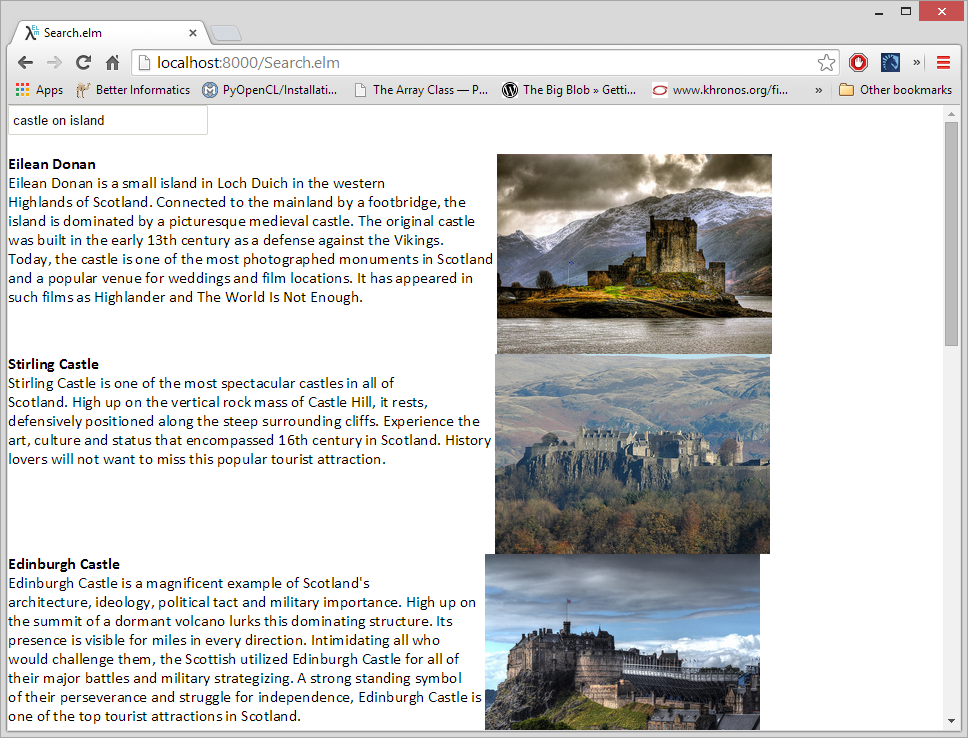
\includegraphics[width=150mm]{castle_island.png}
\caption{Example search engine running using \texttt{elm-reactor}.}
\end{figure}

\begin{figure}[ht!]
\centering
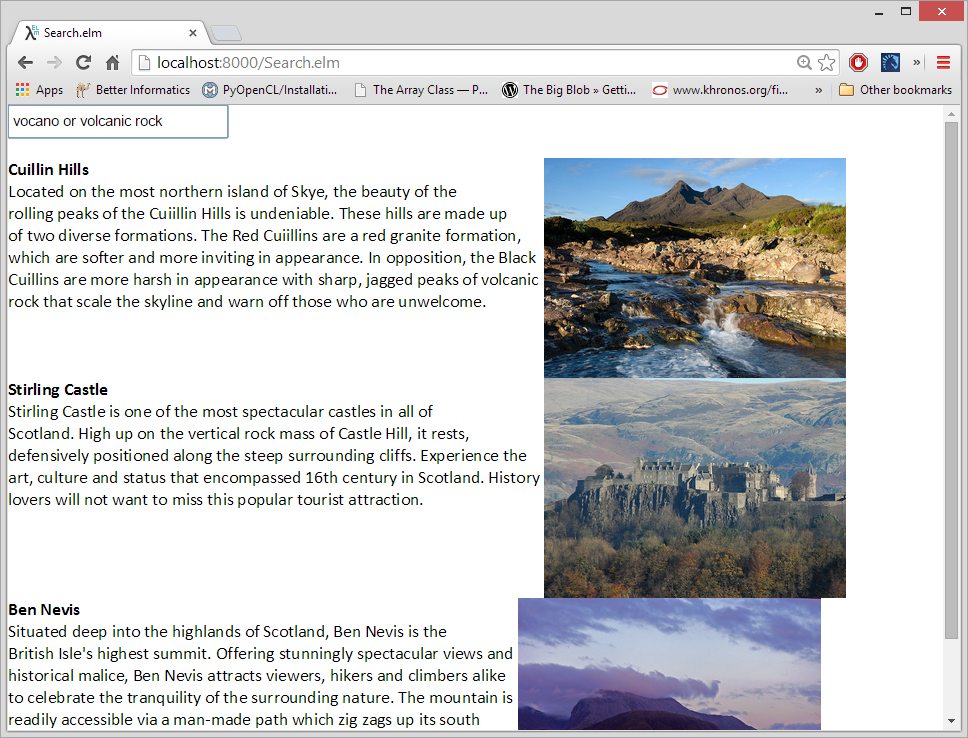
\includegraphics[width=150mm]{volcano_or_volcanic_rock.png}
\caption{A second user query, and its results.}
\end{figure}

\subsection{Implementation}
\subsubsection{Input signal}
The search engine is driven from a single input signal, namely, a \texttt{Graphics.Input.Field} text field input signal:
\begin{samepage}
\begin{verbatim}
import Graphics.Input (Input, input)
import Graphics.Input.Field as Field

searchBar : Input Field.Content
searchBar = input Field.noContent
\end{verbatim}
\end{samepage}
\subsubsection{\texttt{main}}
\label{sec:main}
In \texttt{main}, the above signal is used as input to both a function which yields a signal for the search bar element at the top of the page (\texttt{searchBox}, \texttt{lift}ed) and a function which yields a signal for the result element displayed below (\texttt{scene}, also \texttt{lift}ed). A third, constant newline signal is used to divide the two elements. These
three signals are \texttt{combine}d and laid out by using \texttt{lift (flow down)}, resulting in the \texttt{Signal Element} return value.
\begin{samepage}
\begin{verbatim}
main : Signal Element
main = let search = Field.field Field.defaultStyle searchBar.handle identity
  in
    combine
    [ lift (search "Enter search") searchBar.signal
    , plainText "\n" |> constant
    , dropRepeats searchBar.signal 
      |> sampleOn (every (2 * second)) 
      |> lift scene
    ] |> lift (flow down)
\end{verbatim}
\end{samepage}
\subsubsection{scene}
The \texttt{scene} function takes \texttt{searchBar}'s contents as input. Its tokenized
contents are passed into \texttt{attractionsByRelevance}, which returns a list of 
attractions (\texttt{record}s) sorted by query-relevance (descending). Each of these
is then converted into a "result" element (containing title, description, and image)
by the inline \texttt{result} function. Finally, the individual results are combined
into a single element via \texttt{flow down}.
\begin{samepage}
\begin{verbatim}
scene : Field.Content -> Element
scene fieldContent = 
  let sortedAttractions = tokens fieldContent.string 
                          |> attractionsByRelevance
      result attraction = [ (toText >> bold) attraction.title
                          , toText attraction.body, toText "\n"
                          ] 
                          |> map leftAligned 
                          |> flow down
                          |> flip (::) [image 275 200 attraction.imageUrl]
                          |> flow right
  in 
    map result sortedAttractions |> flow down
\end{verbatim}
\end{samepage}

\subsection{Development}
\begin{figure}[ht!]

\centering
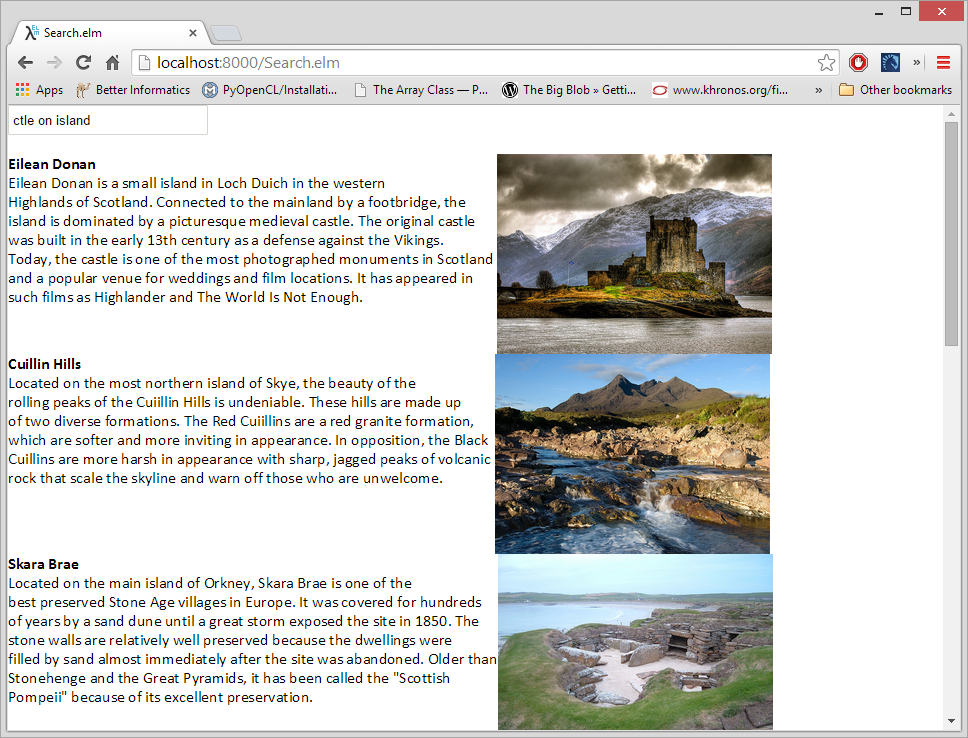
\includegraphics[width=150mm]{lost_input.png}
\caption{User query typed at moderate speed into the text input element is partially discarded.}
\label{fig:Lost}
\end{figure}
Because ranking the attractions by tf-idf score is a nontrivial computation, naively passing the text field's signal directly to \texttt{scene} within \texttt{main} (as below) results in a text field that is not only unresponsive, but, worse, loses user input (see Figure \ref{fig:Lost}).
\begin{samepage}
\begin{verbatim}
let finalElements fieldContent = 
  [ search "Enter search" fieldContent
  , scene fieldContent  -- results in unresponsive text field
  ] |> flow down
in
  lift finalElements searchBar.signal
\end{verbatim}
\end{samepage}
To combat this, the user input signal is instead first filtered down (via \texttt{dropRepeats}) into a signal which contains only events which reflect a change in the input, e.g. from
\begin{samepage}
\begin{verbatim}
- A - A - A - B - B - C - D - D -
\end{verbatim}
to
\begin{verbatim}
- A - - - - - B - - - C - D - - -
\end{verbatim}
\end{samepage}
Further to this, the resultant stream is sampled only once every two seconds - unfortunately, shorter time periods still cause issues with loss of user input. This transformation can be visualized as follows:
\begin{samepage}
\begin{verbatim}
- A - - - - - B - - - C - D - - -
\end{verbatim}
to (assuming five dashes are equivalent to two seconds):
\begin{verbatim}
- - - - A - - - - B - - - - D - -
\end{verbatim}
\end{samepage}
The final process is therefore:
\begin{samepage}
\begin{verbatim}
combine
[ lift (search "Enter search") searchBar.signal
, dropRepeats searchBar.signal  -- keep only changes
  |> sampleOn (every (2 * second))  -- events every two seconds
  |> lift scene  -- pass to scene, which ranks attractions
] |> lift (flow down)
\end{verbatim}
\end{samepage}
Note that this requires "splitting" \texttt{searchBar.signal} (as mentioned in \ref{sec:main}), as otherwise the search engine's text input field would only accept keystrokes every two seconds. The two results of type \texttt{Signal Element} are then put into a list (\texttt{[Signal Element]}), which is transformed into type \texttt{Signal [Element]} by \texttt{combine}.

Were the relevancy rankings a server-side computation requested via AJAX, the resultant signal would have been asynchronous by default, which would allow for displaying the ranked results as soon as they are ready. In Asynchronous Functional Reactive Programming for GUIs, \cite{czaplicki_chong_2013} describe an \texttt{async} primitive for elm which allows any signal to be marked for asynchronous computation, allowing these signals to be arbitrarily computationally expensive without compromising GUI responsiveness. This, however, does not appear in the current implementation of elm.
\section{Resources}

\section{Related work}

\section{Conclusion}

\bibliographystyle{IEEEtranN}
\bibliography{bib}

\begin{appendices}
\chapter{Appendix A: Example source code}
\label{app:A}
\begin{verbatim}
import String
import Char
import Set
import List
import Dict
import Text
import Graphics.Input (Input, input)
import Graphics.Input.Field as Field

-- based on the example given at 
-- http://elm-lang.org/edit/examples/Reactive/TextField.elm 
-- (Accessed 4th November 2014):
searchBar : Input Field.Content
searchBar = input Field.noContent

main : Signal Element
main = let search = Field.field Field.defaultStyle searchBar.handle identity
  in
    combine
    [ lift (search "Enter search") searchBar.signal
    , plainText "\n" |> constant
    , dropRepeats searchBar.signal 
      |> sampleOn (every (2 * second)) 
      |> lift scene
    ] |> lift (flow down)

scene : Field.Content -> Element
scene fieldContent = 
  let sortedAttractions = tokens fieldContent.string 
                          |> attractionsByRelevance
      result attraction = [ (toText >> bold) attraction.title
                          , toText attraction.body, toText "\n"
                          ] 
                          |> map leftAligned 
                          |> flow down
                          |> flip (::) [image 275 200 attraction.imageUrl]
                          |> flow right
  in 
    map result sortedAttractions |> flow down

type Attraction = { title: String, body: String, imageUrl: String }

-- taken from 
-- http://www.touropia.com/tourist-attractions-in-scotland/ 
-- (Accessed 4th November 2014):
attractions : [Attraction]
attractions = 
  [
    {title = "Broch of Mousa",
     body = "One of the most prestigious and well-preserved brochs in the 
Shetland Islands, this impressive structure is a rotund tower lined with 
stone internally and externally to provide the optimum strength as a 
defensive structure. The tower was built around 100 BC and is the only 
broch which is complete right to the top, including the original 
intramural stair.",
     imageUrl = 
      "http://farm2.static.flickr.com/1160/1427611613_a686a1854d_z.jpg?zz=1"
     }
  , {title = "Melrose Abbey",
     body = "Melrose Abbey was founded in 1136 by Cistercian monks, on the 
request of King David I of Scotland. This grand ruin with lavish masonic 
decoration is thought to hold the embalmed heart of Robert the Bruce, 
another king of Scotland. Truly a place of legends, Melrose Abbey is one 
of the most historically significant architectural structures in Scotland.",
     imageUrl = 
      "http://farm4.static.flickr.com/3153/2729634256_863d2b2176_z.jpg?zz=1"
     }
  , {title = "Cuillin Hills",
     body = "Located on the most northern island of Skye, the beauty of the 
rolling peaks of the Cuiillin Hills is undeniable. These hills are made up 
of two diverse formations. The Red Cuiillins are a red granite formation, 
which are softer and more inviting in appearance. In opposition, the Black 
Cuillins are more harsh in appearance with sharp, jagged peaks of volcanic 
rock that scale the skyline and warn off those who are unwelcome.",
     imageUrl = 
      "http://farm3.static.flickr.com/2448/3633666760_f947b66942_z.jpg?zz=1"
     }
  , {title = "Skara Brae",
     body = "Located on the main island of Orkney, Skara Brae is one of the 
best preserved Stone Age villages in Europe. It was covered for hundreds 
of years by a sand dune until a great storm exposed the site in 1850. The 
stone walls are relatively well preserved because the dwellings were 
filled by sand almost immediately after the site was abandoned. Older than
Stonehenge and the Great Pyramids, it has been called the \"Scottish 
Pompeii\" because of its excellent preservation.",
     imageUrl = 
      "http://farm1.static.flickr.com/96/251621816_f4d2c13d90_z.jpg?zz=1"
     }
  , {title = "Stirling Castle",
     body = "Stirling Castle is one of the most spectacular castles in all of 
Scotland. High up on the vertical rock mass of Castle Hill, it rests, 
defensively positioned along the steep surrounding cliffs. Experience the 
art, culture and status that encompassed 16th century in Scotland. History 
lovers will not want to miss this popular tourist attraction.",
     imageUrl = 
      "http://farm1.static.flickr.com/183/483655010_d9c9794fbd_z.jpg?zz=1"
     }
  , {title = "Luskentyre Beach",
     body = "Luskentyre beach is situated on the spectacular west coast of 
South Harris in the Outer Hebrides. One of the most beautiful 
color-washed coastal areas of Scotland, its blue-green seas shimmer 
against creamy sands and the vibrant green hillside. Peaceful and 
timeless, Luskentyre Beach has been voted Britain's best beach.",
     imageUrl = 
      "http://farm6.static.flickr.com/5191/5902560358_914edfa75e_z.jpg?zz=1"
     }
  , {title = "Loch Ness",
     body = "One of the most famous lakes in the world, Loch Ness is the second 
largest loch in Scotland after Loch Lomond (and due to its great depth it 
is the largest by volume). About a mile wide at most places it holds the 
legend of an infamous sea monster. The most notorious mythical creature of 
modern time, Nessie, is said to dwell in the lake. With an air of mystery, 
the intriguing area of Loch Ness should not be missed. You might even get 
a glimpse of Nessie!",
     imageUrl = 
      "http://farm3.static.flickr.com/2712/4441473182_a5125fec3e_z.jpg?zz=1"
     }
  , {title = "Ben Nevis",
     body = "Situated deep into the highlands of Scotland, Ben Nevis is the 
British Isle's highest summit. Offering stunningly spectacular views and 
historical malice, Ben Nevis attracts viewers, hikers and climbers alike 
to celebrate the tranquility of the surrounding nature. The mountain is 
readily accessible via a man-made path which zig zags up its south 
westerly face, while the rock face on the north west of the mountain is 
strictly for experienced mountaineers only.",
     imageUrl = 
      "http://farm5.static.flickr.com/4154/4963323610_47f0ebdef4_z.jpg?zz=1"
     }
  , {title = "Eilean Donan",
     body = "Eilean Donan is a small island in Loch Duich in the western 
Highlands of Scotland. Connected to the mainland by a footbridge, the 
island is dominated by a picturesque medieval castle. The original castle 
was built in the early 13th century as a defense against the Vikings. 
Today, the castle is one of the most photographed monuments in Scotland 
and a popular venue for weddings and film locations. It has appeared in 
such films as Highlander and The World Is Not Enough.",
     imageUrl = 
      "https://c2.staticflickr.com/4/3293/2433869373_15e31d33d2_z.jpg?zz=1"
     }
  , {title = "Edinburgh Castle",
     body = "Edinburgh Castle is a magnificent example of Scotland's 
architecture, ideology, political tact and military importance. High up on 
the summit of a dormant volcano lurks this dominating structure. Its 
presence is visible for miles in every direction. Intimidating all who 
would challenge them, the Scottish utilized Edinburgh Castle for all of 
their major battles and military strategizing. A strong standing symbol 
of their perseverance and struggle for independence, Edinburgh Castle is 
one of the top tourist attractions in Scotland.",
     imageUrl = 
      "https://c4.staticflickr.com/8/7386/9550271050_32bf1bf589_c.jpg?zz=1"
     }
  ]
  
alphanumericCharacters = String.toList "abcdefghijklmnopqrstuvwxyz0123456789"
                         |> Set.fromList 
  
startingLetters : String -> String
startingLetters string = let isAlnum = flip Set.member alphanumericCharacters
  in
    String.toList string  
    |> List.partition isAlnum
    |> fst >> String.fromList
  
tokens : String -> [String]
tokens string = String.words string 
                |> map String.toLower 
                |> map startingLetters

unique : [String] -> [String]
unique xs = Set.fromList xs |> Set.toList 

counts : [String] -> Dict.Dict String Int
counts tokens = let uniqueTokens = unique tokens
                    count item list = List.filter ((==) item) list 
                                      |> List.length
                    tokenCount = flip count tokens
  in
    map tokenCount uniqueTokens 
    |> zip uniqueTokens 
    |> Dict.fromList

-- tf-idf algorithm adapted from personal previous coursework for
-- Text Technologies for Data Science (INFR11100)
-- Assessment 1, 6th October 2014
idf : String -> Float
idf token = let documents = map (.body >> tokens >> Set.fromList) attractions
                tokenFrequency = filter (Set.member token) documents 
                                 |> List.length
  in 
     toFloat (List.length attractions) / toFloat tokenFrequency |> logBase 2
    
relevance : [String] -> [String] -> Float
relevance query document = 
  let mutualTokens = (Set.fromList query, Set.fromList document) 
                     |> uncurry Set.intersect 
                     |> Set.toList
      queryCounts = counts query
      queryCount token = Dict.getOrElse 0 token queryCounts |> toFloat
      documentCount token = Dict.getOrElse 0 token documentCounts |> toFloat
      documentCounts = counts document
      k = 2
      documents = map (.body >> tokens) attractions
      averageK = (sum >> toFloat) (map length documents) 
                 / (length >> toFloat) documents
      documentSquash token = documentCount token 
                             + (averageK * toFloat (length document))
      tfidf token = queryCount token * documentCount token 
                    / documentSquash token * idf token
  in
    map tfidf mutualTokens |> sum
    
attractionsByRelevance : [String] -> [Attraction]
attractionsByRelevance query = attractions
                               |> map (.body >> tokens >> relevance query)
                               |> flip zip attractions
                               |> filter (fst >> (<) 0)
                               |> List.sortBy fst
                               |> List.reverse 
                               |> map snd
\end{verbatim}

\end{appendices}

\end{document}